\documentclass{article}
\usepackage{tikz}
\usetikzlibrary{calc}

\begin{document}
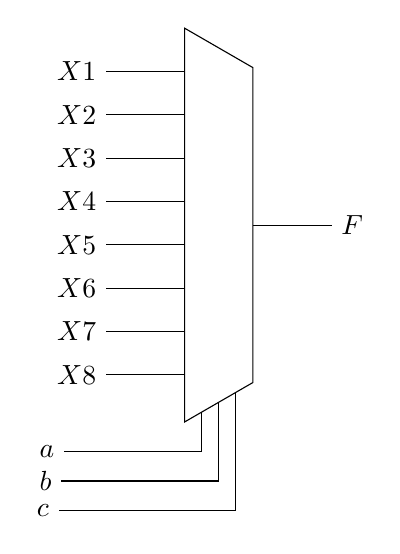
\begin{tikzpicture}
\draw (0,0)coordinate (O)--++(30:1)coordinate (A)--++(90:4)coordinate (B)--++(150:1)coordinate (C)--cycle;
\draw ($(A)!0.5!(B)$)--++(0:1)node[right]{$F$};
\draw ($(O)!0.5!(A)$)--++(-90:1)--++(180:2)node[left]{$b$};
\draw ($(O)!0.25!(A)$)--++(-90:0.5)--++(180:1.75)node[left]{$a$};
\draw ($(O)!0.75!(A)$)--++(-90:1.5)--++(180:2.25)node[left]{$c$};
\foreach \y/\t in {0.1/1,0.2/2,0.3/3,0.4/4,0.5/5,0.6/6,0.7/7,0.8/8} {
\draw ($(C)! \y*1.1 !(O)$)--++(180:1) node[left] {$X \t$};}
\end{tikzpicture}

\end{document}